%!TEX program = lualatex
\documentclass[a4paper,14pt]{extarticle}

% === Кодировка и язык ===
\usepackage{fontspec}
\usepackage[russian]{babel}
% Иначе символ " активен и ломает \texttt{"..."} в тексте
\AtBeginDocument{\shorthandoff{"}}
% DejaVu: полная кириллица; сборка через lualatex обходит сбой xdvipdfmx на pfb у некоторых конфигураций
\defaultfontfeatures{Ligatures=TeX}
\setmainfont{DejaVu Serif}
\setsansfont{DejaVu Sans}
\setmonofont{DejaVu Sans Mono}

% === Геометрия страницы ===
\usepackage{geometry}
\geometry{
  a4paper,
  left=30mm, right=15mm,
  top=20mm, bottom=20mm
}

% === Межстрочный интервал ===
\usepackage{setspace}
\onehalfspacing

% === Оглавление и заголовки ===
\usepackage{titlesec}
\titleformat{\section}{\normalfont\large\bfseries}{\thesection.}{0.5em}{}
\titleformat{\subsection}{\normalfont\normalsize\bfseries}{\thesubsection.}{0.5em}{}

% === Колонтитулы ===
\usepackage{fancyhdr}
\setlength{\headheight}{17pt}
\pagestyle{fancy}
\fancyhf{}
\fancyhead[R]{\thepage}
\renewcommand{\headrulewidth}{0pt}

% === Работа с рисунками, таблицами, листингами ===
\usepackage{graphicx}
\usepackage{caption}
\usepackage{listings}
% Для листингов с breaklines=true (C): без выключки и без «лестницы» переносов
\lstset{breakautoindent=false,breakindent=0pt}
\makeatletter
\lst@AddToHook{Init}{\raggedright}
\makeatother
\usepackage{xcolor}
\usepackage{tabularx}
\usepackage{booktabs}
\usepackage{array}
\usepackage{longtable}
\usepackage{float}

% === Листинги кода (как в report/4; переносы — только по пробелам для PL/1 и ASM) ===
\lstdefinestyle{Cstyle}{
  language=C,
  basicstyle=\small\ttfamily,
  keywordstyle=\bfseries\color{black},
  commentstyle=\itshape\color{gray},
  stringstyle=\color{black},
  numbers=left,
  numberstyle=\tiny,
  stepnumber=1,
  numbersep=6pt,
  breaklines=true,
  frame=single,
  tabsize=2,
  showstringspaces=false,
  extendedchars=true
}

% PL/1 и ASM в отчёте: без автопереноса — подставляются заранее разбитые файлы snippets/*
\lstdefinestyle{ASMstyle}{
  basicstyle=\small\ttfamily,
  numbers=none,
  breaklines=false,
  frame=single,
  tabsize=8,
  showstringspaces=false
}

\lstdefinestyle{PLIstyle}{
  basicstyle=\small\ttfamily,
  numbers=none,
  breaklines=false,
  frame=single,
  showstringspaces=false
}

% === Гиперссылки ===
\usepackage[hidelinks]{hyperref}
% Пути к файлам: \texttt + \detokenize (совместимо с listings / fontspec)
\newcommand{\fpath}[1]{\texttt{\detokenize{#1}}}

% === Прочее ===
\usepackage{enumitem}
\usepackage{amsmath}
\usepackage{indentfirst}
\setlength{\parindent}{1.25cm}
% Нетерминал в math: \text{PRO} с polyglossia/fontspec часто даёт пустые латинские буквы
\newcommand{\NT}[1]{\langle\mathrm{#1}\rangle}

% === Подписи к рисункам (как в этапах 1–4) ===
\captionsetup[figure]{name=Рис.,labelsep=period}
\captionsetup[table]{name=Таблица,labelsep=period}

\begin{document}
\sloppy
\emergencystretch=2em

% ============================================================
% ТИТУЛЬНЫЙ ЛИСТ
% ============================================================
\thispagestyle{empty}
\begin{center}
  \textbf{Санкт-Петербургский политехнический университет}\\
  \textbf{Институт компьютерных наук и технологий}\\
  \textbf{Высшая школа программной инженерии}\\[3cm]

  {\Large\textbf{К У Р С О В А Я \quad Р А Б О Т А}}\\[1cm]
  {\large Разработка учебной системы программирования}\\[0.5cm]
  {\large Компилятор с ЯВУ}\\[2cm]

  Дисциплина: «Системы программирования»\\[1cm]
  Вариант~№~11\\[2cm]
\end{center}

\begin{flushright}
  \begin{tabular}{ll}
    Исполнители: & Студенты группы~5140904/50102\\
                 & Сырбу~Г.~В.\\
                 & Федерова~С.~К.\\[0.5cm]
    Руководитель: & Расторгуев~В.~Я.\\
  \end{tabular}
\end{flushright}

\vfill
\begin{center}
  Санкт-Петербург\\
  2026
\end{center}

\newpage

% ============================================================
% СОДЕРЖАНИЕ
% ============================================================
\tableofcontents
\newpage

% ============================================================
% РАЗДЕЛ 1. ЗАДАНИЕ НА КУРСОВУЮ РАБОТУ
% ============================================================
\section{Задание на курсовую работу}

Задание на курсовую работу дано в следующей общей формулировке:

\begin{quote}
«Необходимо выполнить доработку элементов макета учебной системы
программирования до уровня, позволяющего обрабатывать «новые» для макета
конструкции языка высокого уровня, примененные в соответствующем варианте».
\end{quote}

Общая формулировка персонализирована в варианте~№~11. Исходная постановка задания
содержала один оператор \texttt{C = A = (B * 5);} в теле процедуры. По согласованию
с преподавателем вложенное выражение со скобками заменено двумя последовательными
операторами присваивания; актуальный исходный текст персонального варианта хранится
в файле \fpath{input/ex11.pli} (рис.~\ref{fig:variant_mod}).

\begin{figure}[H]
\centering
\lstinputlisting[style=PLIstyle]{snippets/ex11_display.pli}
\caption{Персональный вариант~№~11 (\fpath{input/ex11.pli}; в отчёте — тот же текст из \fpath{snippets/ex11_display.pli} без полей пробелов 80-колоночной разрядки)}
\label{fig:variant_mod}
\end{figure}

Схема функционирования макета учебной системы программирования приведена на
рис.~\ref{fig:arch}. Согласно заданию на КР этот макет входит в число элементов
исходных данных.

\begin{figure}[H]
\centering
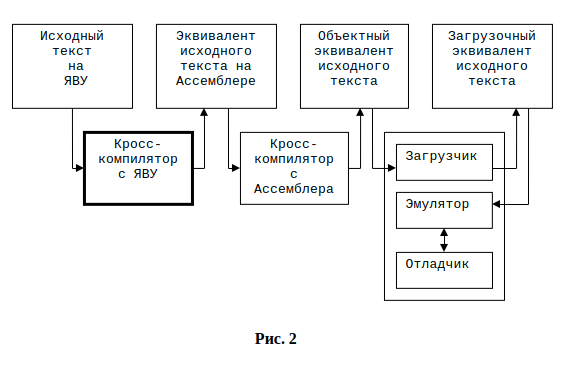
\includegraphics[width=\textwidth]{../источники/image.png}
\caption{Схема функционирования учебной системы программирования}
\label{fig:arch}
\end{figure}

Дополнительные требования к КР предполагают, что данная система программирования
работает на технологической ЭВМ (IBM PC) и является по существу кросс-системой для
объектной ЭВМ (IBM~370). В этой системе:
\begin{itemize}
  \item в качестве языка высокого уровня (ЯВУ) выбран язык, образованный из
        подмножества языковых конструкций PL/1; исходная программа готовится в виде
        текстового файла с расширением \texttt{*.pli};
  \item язык Ассемблера сформирован из языковых конструкций Ассемблера IBM~370;
        ассемблерный эквивалент исходной программы формируется в виде текстового
        файла с расширением \texttt{*.ass};
  \item объектный эквивалент исходной программы готовится в формате объектных файлов
        ОС IBM~370 и хранится в виде двоичного файла с расширением \texttt{*.tex};
  \item загрузочный эквивалент исходной программы представляет собой машинный код
        IBM~370, запоминаемый в области ОЗУ технологической ЭВМ; эта область служит
        зоной загрузки для эмулятора объектной ЭВМ.
\end{itemize}

В данном отчёте документируются результаты модификации макетного компилятора с~ЯВУ
под персональный вариант~№~11.

\subsection*{Контрольный (демонстрационный) пример}

Контрольным примером, на который изначально настроен макет компилятора,
является программа \texttt{examppl.pli} (рис.~\ref{fig:demo}).

\begin{figure}[H]
\centering
\lstinputlisting[style=PLIstyle]{snippets/examppl_display.pli}
\caption{Демонстрационный пример (\fpath{input/examppl.pli}; для отчёта — \fpath{snippets/examppl_display.pli})}
\label{fig:demo}
\end{figure}

\subsection*{Отличия персонального варианта от демонстрационного примера}

При сравнении файлов \fpath{input/ex11.pli} и \fpath{input/examppl.pli}
(рис.~\ref{fig:variant_mod} и рис.~\ref{fig:demo}) выявлены следующие отличия:

\begin{enumerate}[leftmargin=*,itemsep=0.35em]
  \item В \fpath{input/examppl.pli} для всех объявлений \texttt{BIN FIXED} указана
        разрядность \texttt{(31)}, инициализация задана двоичными литералами
        \texttt{11B}, \texttt{100B}, \texttt{101B}. В \fpath{input/ex11.pli} для
        \texttt{BIN FIXED} указана разрядность \texttt{(15)}, инициализация
        \texttt{A} и \texttt{B} задана литералом \texttt{11B} (двоичная запись
        значения~3).

  \item В \fpath{input/ex11.pli} переменная \texttt{B} объявлена как
        \texttt{DEC FIXED (3)}; в \fpath{input/examppl.pli} все переменные —
        \texttt{BIN FIXED}.

  \item Оператор \texttt{C = B * 5;} в \fpath{input/ex11.pli} использует «\texttt{*}»
        для умножения упакованного десятичного \texttt{B} на однозначный
        десятичный множитель \texttt{5}. В \fpath{input/examppl.pli} операция
        «\texttt{*}» не встречается.

  \item Оператор \texttt{C = A = C;} в \fpath{input/ex11.pli} задаёт сравнение
        \texttt{A} и \texttt{C} во второй позиции присваивания; в формальной
        грамматике (разд.~3) правая часть моделируется как \texttt{<AVL>}, оператор
        --- как \texttt{<OPL>}. В \fpath{input/examppl.pli} такой конструкции нет.
\end{enumerate}

% ============================================================
% РАЗДЕЛ 2. ПОСТАНОВКА ЗАДАЧИ
% ============================================================
\section{Постановка задачи модификации макета в части компилятора с ЯВУ}

Схема функционирования модифицированного макетного компилятора с~ЯВУ должна
соответствовать рис.~\ref{fig:compil_scheme}.

\begin{figure}[H]
\centering
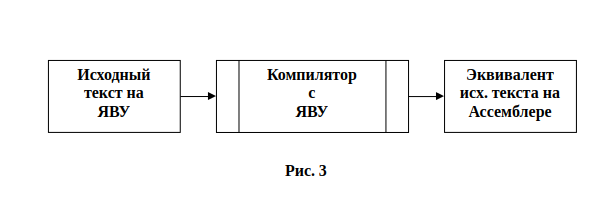
\includegraphics[width=\textwidth]{../источники/image2.png}
\caption{Схема функционирования модифицированного макетного компилятора с~ЯВУ}
\label{fig:compil_scheme}
\end{figure}

Функционал модифицированного макетного компилятора должен обеспечить компиляцию
исходного текста на ЯВУ (рис.~\ref{fig:variant_mod}) в эквивалент исходного текста на
Ассемблере, представленный на рис.~\ref{fig:etalon}.

\begin{figure}[H]
\centering
\lstinputlisting[style=ASMstyle]{snippets/ex11_display.ass}
\caption{Эталон ассемблерного эквивалента (\fpath{report/5/etalon/ex11.ass}; для отчёта — \fpath{snippets/ex11_display.ass}, по строкам как в листинге)}
\label{fig:etalon}
\end{figure}

\subsection*{Согласованные функциональные ограничения}

По согласованию с преподавателем в модифицированном макетном компиляторе сохраняются
и уточняются следующие ограничения (согласованы с программой рис.~\ref{fig:variant_mod} и эталоном рис.~\ref{fig:etalon}):

\begin{enumerate}[leftmargin=*,itemsep=0.35em]
  \item Компилятор не задаёт повышенный приоритет умножения в \texttt{<AVI>}: вычисление ведётся
        последовательно слева направо для операций «\texttt{+}», «\texttt{-}», «\texttt{*}».

  \item В операторе \texttt{C = B * 5;} (файл \fpath{input/ex11.pli}) множитель \texttt{5} ---
        одна десятичная цифра. В секции данных для него резервируется упакованная константа
        \texttt{@FIVE} (рис.~\ref{fig:etalon}).

  \item Сравнение в операторе \texttt{C = A = C;} оформлено как \texttt{<AVL>} с операндами
        \texttt{A} и \texttt{C} (оба \texttt{BIN FIXED} в \fpath{input/ex11.pli}). Результат сравнения
        --- \texttt{0} или \texttt{1} в полуслове; записывается в~\texttt{C}.
\end{enumerate}

% ============================================================
% РАЗДЕЛ 3. МОДИФИКАЦИЯ БД КОМПИЛЯТОРА
% ============================================================
\section{Модификация состава и структуры БД макета компилятора с ЯВУ}

\subsection{Модификация БД лексического анализатора}

БД лексического анализатора определяется путём выделения подмножества терминальных
символов-разделителей термов языка. Функция лексического анализа в макете реализована
в подпрограмме \texttt{compress\_ISXTXT()}.

Для персонального варианта~№~11 разделителями термов являются терминальные символы
из множества:
\[
  \{\,\texttt{":"}\,,\, \texttt{"("}\,,\, \texttt{")"}\,,\, \texttt{";"}\,,\,
     \texttt{"+"}\,,\, \texttt{"-"}\,,\, \texttt{"="}\,,\, \texttt{"\_"}\,,\,
     \texttt{"*"}\,\}
\]

Модификация лексических настроек демонстрационного примера состоит в добавлении
символа умножения «\texttt{*}» в перечень разделителей термов. Данный символ в
оригинальном макете не входил в число обрабатываемых разделителей. Поскольку авторы
макета разместили перечень символов-разделителей непосредственно в теле подпрограммы
\texttt{compress\_ISXTXT()}, модификация выполнена в теле этой подпрограммы:

\begin{lstlisting}[style=Cstyle,caption={Фрагмент \texttt{compress\_ISXTXT()} с добавленным символом «\texttt{*}»},label=lst:lex]
void compress_ISXTXT()
{
  /* ... */
  if (
    ( ISXTXT[I1][I2] == '+' ||
      ISXTXT[I1][I2] == '-' ||
      ISXTXT[I1][I2] == '=' ||
      ISXTXT[I1][I2] == '(' ||
      ISXTXT[I1][I2] == ')' ||
      ISXTXT[I1][I2] == '*'   /* <- добавлен разделитель '*' */
    )
    && PREDSYM == ' '
  )
  { I3--; goto L1; }

  if ( ISXTXT[I1][I2] == ' ' &&
     ( PREDSYM == '+' || PREDSYM == '-' ||
       PREDSYM == '=' || PREDSYM == '*'   /* <- добавлен '*' */
     )
  )
  { goto L2; }
  /* ... */
}
\end{lstlisting}

\subsection{Модификация БД синтаксического анализатора}

Высокоуровневое определение модифицированного синтаксиса для персонального
варианта~№~11 приведено ниже; модификации по сравнению с грамматикой
демонстрационного примера выделены курсивом:

\begin{enumerate}
  \item $\NT{PRO} ::= \NT{OPR}\NT{TEL}\NT{OEN}$
  \item $\NT{OPR} ::= \NT{IPR}\texttt{:PROC\_OPTIONS(MAIN);}$
  \item $\NT{IPR} ::= \NT{IDE}$
  \item $\NT{IDE} ::= \NT{BUK} \mid \NT{IDE}\NT{BUK} \mid \NT{IDE}\NT{CIF}$
  \item $\NT{BUK} ::= \texttt{A} \mid \texttt{B} \mid \texttt{C} \mid \texttt{D} \mid \texttt{E} \mid \texttt{M} \mid \texttt{P} \mid \texttt{X}$
  \item $\NT{CIF} ::= \texttt{0} \mid \texttt{1} \mid \texttt{2} \mid \texttt{3} \mid \texttt{4} \mid \texttt{5} \mid \texttt{6} \mid \texttt{7} \mid \texttt{8} \mid \texttt{9}$
  \item $\NT{TEL} ::= \NT{ODC} \mid \NT{TEL}\NT{ODC} \mid \NT{TEL}\NT{OPA} \mid \NT{TEL}\NT{OPL}$
  \item $\NT{ODC} ::= \texttt{DCL\_}\NT{IPE}\texttt{\_BIN\_FIXED(}\NT{RZR}\texttt{);}$\\
        $\mid\; \texttt{DCL\_}\NT{IPE}\texttt{\_BIN\_FIXED(}\NT{RZR}\texttt{)INIT(}\NT{LIT}\texttt{);}$\\
        \textit{$\mid\; \texttt{DCL\_}\NT{IPE}\texttt{\_BIN\_FIXED;}$}\\
        \textit{$\mid\; \texttt{DCL\_}\NT{IPE}\texttt{\_BIN\_FIXED\_INIT(}\NT{LID}\texttt{);}$}\\
        \textit{$\mid\; \texttt{DCL\_}\NT{IPE}\texttt{\_DEC\_FIXED\_INIT(}\NT{LID}\texttt{);}$}
  \item $\NT{IPE} ::= \NT{IDE}$
  \item $\NT{RZR} ::= \NT{CIF} \mid \NT{RZR}\NT{CIF}$
  \item $\NT{LIT} ::= \NT{MAN}\texttt{B}$
  \item $\NT{MAN} ::= \texttt{1} \mid \NT{MAN}\texttt{0} \mid \NT{MAN}\texttt{1}$
  \item \textit{$\NT{LID} ::= \NT{CIF} \mid \NT{LID}\NT{CIF}$}
  \item $\NT{OPA} ::= \NT{IPE}\texttt{=}\NT{AVI}\texttt{;}$
  \item $\NT{AVI} ::= \NT{LIT} \mid \NT{LID} \mid \NT{IPE}$\\
        $\mid\; \NT{AVI}\NT{ZNK}\NT{LIT}
        \mid \NT{AVI}\NT{ZNK}\NT{LID}
        \mid \NT{AVI}\NT{ZNK}\NT{IPE}$
  \item $\NT{AVL} ::= \NT{AVI}\NT{ZNL}\NT{LIT}
        \mid \NT{AVI}\NT{ZNL}\NT{LID}
        \mid \NT{AVI}\NT{ZNL}\NT{IPE}$
  \item $\NT{OPL} ::= \NT{IPE}\texttt{=}\NT{AVL}\texttt{;}$
  \item $\NT{ZNK} ::= \texttt{+} \mid \texttt{-}$ \textit{$\mid\; \texttt{*}$}
  \item \textit{$\NT{ZNL} ::= \texttt{=}$}
  \item $\NT{OEN} ::= \texttt{END\_}\NT{IPR}$
\end{enumerate}

Пояснения к метасимволам:
\begin{itemize}
  \item \texttt{<} и \texttt{>} — ограничители нетерминального символа;
  \item \texttt{::=} — «равно по определению»;
  \item \texttt{|} — альтернативное определение («или»);
  \item \texttt{\_} — терминальный символ «пробел».
\end{itemize}

Перечень нетерминальных символов приведён в таблице~\ref{tab:nonterm}.

\begin{table}[H]
\centering
\caption{Нетерминальные символы грамматики}
\label{tab:nonterm}
\begin{tabularx}{\textwidth}{|l|X|}
  \hline
  \textbf{Нетерминал} & \textbf{Смысл} \\
  \hline
  \texttt{<PRO>} & программа \\
  \texttt{<OPR>} & оператор пролога программы \\
  \texttt{<IPR>} & имя программы \\
  \texttt{<IDE>} & идентификатор \\
  \texttt{<BUK>} & буква \\
  \texttt{<CIF>} & цифра \\
  \texttt{<TEL>} & тело программы \\
  \texttt{<ODC>} & оператор объявления переменных (DCL) \\
  \texttt{<IPE>} & имя переменной \\
  \texttt{<RZR>} & разрядность \\
  \texttt{<LIT>} & двоичный литерал \\
  \texttt{<MAN>} & мантисса литерала \\
  \texttt{<LID>} & десятичный целочисленный литерал \\
  \texttt{<OPA>} & оператор присваивания (арифметическое выражение) \\
  \texttt{<OPL>} & оператор присваивания (логическое выражение) \\
  \texttt{<AVI>} & арифметическое выражение \\
  \texttt{<AVL>} & логическое выражение \\
  \texttt{<ZNK>} & знак арифметической операции \\
  \texttt{<ZNL>} & знак логической операции \\
  \texttt{<OEN>} & оператор эпилога программы (END) \\
  \hline
\end{tabularx}
\end{table}

По сравнению с грамматикой демонстрационного примера модифицированы правила:
\begin{itemize}[leftmargin=*,itemsep=0.35em]
  \item \textbf{Правило~7 (\texttt{<TEL>}):} в формальной записи добавлена альтернатива
        \texttt{<TEL><OPL>}. В таблице \texttt{SINT[]} для нетерминала \texttt{TEL}
        заданы только ветви с \texttt{ODC} и \texttt{OPA}; отдельного значения
        \texttt{DER="OPL"} в \texttt{VXOD[]} нет. Операторы вида \texttt{C = A = C;}
        разбираются как \texttt{<OPA>}: цепочка \texttt{IPE = AVI ;}, а сравнение во
        второй части присваивания обрабатывается внутри \texttt{<AVI>} при встрече
        второго «\texttt{=}» как элемента \texttt{ZNK} (записи \texttt{SINT[]}
        226--228, вход «\texttt{=}» в \texttt{VXOD[]} с \texttt{VX}=226).

  \item \textbf{Правило~8 (\texttt{<ODC>}):} для файлов \fpath{input/examppl.pli} и
        \fpath{input/ex11.pli} используются объявления \texttt{BIN FIXED} и
        \texttt{DEC FIXED} с явной разрядностью в скобках; инициализация задаётся
        двоичными литералами \texttt{<LIT>} (\texttt{11B} и~т.\,п.) в обоих примерах
        там, где в исходнике указано \texttt{INIT ( \ldots B )}.

  \item \textbf{Правило~13 (\texttt{<LID>}):} нетерминал описывает цепочки цифр для
        десятичной записи (в т.\,ч.\ множитель \texttt{5} в \texttt{C = B * 5;}).

  \item \textbf{Правила~15--17 (\texttt{<AVI>}, \texttt{<AVL>}, \texttt{<OPL>}):}
        расширен \texttt{<AVI>}, введены \texttt{<AVL>} и \texttt{<OPL>} для модели
        сравнения и присваивания булева результата.

  \item \textbf{Правило~18 (\texttt{<ZNK>}):} добавлен знак «\texttt{*}».

  \item \textbf{Правило~19 (\texttt{<ZNL>}):} введён знак сравнения «\texttt{=}»,
        не смешиваемый с арифметическими «\texttt{+}»/«\texttt{-}»/«\texttt{*}» в
        одном нетерминале \texttt{<ZNK>}.
\end{itemize}

В состав нетерминальных символов после модификации добавлены нетерминалы
\texttt{<LID>} (десятичный целочисленный литерал), \texttt{<ZNL>} (знак
логической операции), \texttt{<AVL>} (логическое выражение) и \texttt{<OPL>}
(оператор присваивания с логическим выражением).

\subsubsection*{Модификация таблицы синтаксических правил \texttt{SINT[]}}

Таблица \texttt{SINT[]} реализует двунаправленный список с альтернативными
ветвлениями, в котором каждая запись описывает один шаг распознавания (форма
распознавания — от правой части к нетерминалу). В ходе модификации:

\begin{itemize}
  \item задано \texttt{\#define NSINT~232}; добавлены ветви \texttt{DEC FIXED} (201--225),
        «\texttt{*}» (198--200), «\texttt{=}» в выражении (226--228), операнд \texttt{RZR} в \texttt{AVI} (229--231);
        изменено поле \texttt{ALT} у записи~168;
  \item в \texttt{VXOD[]}: для «\texttt{*}» поле \texttt{VX}=198, для «\texttt{=}» --- \texttt{VX}=226;
  \item в \texttt{TPR[][]} обновлены отношения для «\texttt{*}», «\texttt{=}» и \texttt{ZNK}.
\end{itemize}

\subsubsection*{Связь грамматики разд.~3 с реализацией}

Нетерминалы \texttt{<LID>}, \texttt{<ZNL>}, \texttt{<AVL>}, \texttt{<OPL>} задают
учебную модель языка. В программе \fpath{src/komppl.c} отдельные строки \texttt{VXOD[]}
для имён \texttt{LID}, \texttt{ZNL}, \texttt{AVL}, \texttt{OPL} не используются:
десятичные цифры множителя в \texttt{C = B * 5;} распознаются как терминалы
\texttt{CIF}, сравнение во втором «\texttt{=}» --- через записи \texttt{SINT[]}
226--228 и элемент \texttt{VXOD[]} для лексемы «\texttt{=}» (\texttt{VX}=226), что
семантически соответствует \texttt{<AVL>} и \texttt{<ZNL>}. Семантика присваивания
(включая запись результата сравнения) вызывается для \texttt{OPA} второго прохода
--- функция \texttt{OPA2()}; отдельной функции \texttt{OPL2()} нет.

Для ветви \texttt{DEC FIXED \ldots INIT(\ldots)} в \texttt{SINT[]} в правой части
инициализации стоит распознавание через нетерминал \texttt{LIT} (см.\ записи
с \texttt{DER="LIT"} после \texttt{INIT}), а не через отдельную ветку \texttt{LID}.
Семантика \texttt{ODC1()} записывает строку инициализации в \texttt{SYM[].INIT};
для \texttt{DEC FIXED} значение интерпретируется по контексту объявления.

% ============================================================
% РАЗДЕЛ 4. МОДИФИКАЦИЯ АЛГОРИТМА
% ============================================================
\section{Модификация алгоритма макета компилятора с ЯВУ}

Реализация находится в файле \fpath{src/komppl.c} каталога \fpath{lab-step-1-1}.
Ключевые функции второго прохода:

\begin{itemize}
  \item \textbf{\texttt{ODC1()}} --- типы \texttt{BIN}/\texttt{DEC FIXED}, таблица \texttt{SYM[]}, инициализация;
  \item \textbf{\texttt{AVI2()}} --- операнды, \texttt{+}/\texttt{-}/\texttt{*}, \texttt{ZAP}/\texttt{MP}/\texttt{CVB}; при \texttt{op\_sign == '='}
        вызывается \texttt{avl2\_emit\_compare\_rhs()};
  \item \textbf{\texttt{avl2\_emit\_compare\_rhs()}} --- генерация сравнения (рис.~\ref{fig:etalon});
  \item \textbf{\texttt{OPA2()}} --- \texttt{STH} и \texttt{PENDING\_LABEL} (и для арифметики, и для булева результата);
  \item \textbf{\texttt{OEN2()}} --- секция данных, \texttt{EXTRA[]}, \texttt{@BUF}, \texttt{END};
  \item \textbf{\texttt{OPR2()}} --- \texttt{START}, \texttt{BALR}, \texttt{USING}.
\end{itemize}

Используются \texttt{SETCOMM()}, \texttt{const\_label()}, глобальные \texttt{RESULT\_REG}, \texttt{PENDING\_LABEL}, \texttt{EXTRA[]}
(листинг~\ref{lst:globals4}).

\begin{lstlisting}[style=Cstyle,caption={Фрагмент \texttt{komppl.c}},label=lst:globals4]
char RESULT_REG[9] = "@R2";
char PENDING_LABEL[9] = "";
struct { char name[9]; char type; int size; char value[10]; } EXTRA[20];
int NEXTRA = 0;
static void avl2_emit_compare_rhs ( const char *rhs_name ) { /* ... */ }
\end{lstlisting}

% ============================================================
% РАЗДЕЛ 5. РЕЗУЛЬТАТЫ ЭКСПЕРИМЕНТАЛЬНОЙ ПРОВЕРКИ
% ============================================================
\section{Результаты экспериментальной проверки модифицированного компилятора с ЯВУ}

Работоспособность подтверждается сборкой в среде Linux (\texttt{gcc~-m32}): см.\
\fpath{README.md} и \fpath{Makefile} в каталоге \fpath{lab-step-1-1}. Рекомендуемый
запуск --- из Docker-образа по \fpath{Dockerfile} в корне репозитория (монтирование
каталога \fpath{lab-step-1-1} в \texttt{/lab}).

\begin{lstlisting}[style=Cstyle,basicstyle=\small\ttfamily,caption={Сборка и проверка в каталоге \fpath{lab-step-1-1}},label=lst:build4]
make
make check
\end{lstlisting}

Цель \texttt{make check} запускает \texttt{build/komppl.exe} для файлов
\fpath{input/ex11.pli} и \fpath{input/examppl.pli}. Ассемблерный текст записывается
рядом с исходником: \fpath{input/ex11.ass}, \fpath{input/examppl.ass}. Сравнение
выполняется с эталонами \fpath{report/5/etalon/ex11.ass} и
\fpath{report/5/etalon/examppl.ass}. Эталонный листинг для \texttt{ex11} --- на
рис.~\ref{fig:etalon}; цель \texttt{make check} подтверждает побайтовое совпадение
\fpath{input/ex11.ass} с \fpath{report/5/etalon/ex11.ass}.

\subsection*{Пояснения к сгенерированному тексту}

\textbf{Семантика \fpath{input/ex11.pli}} (рис.~\ref{fig:variant_mod}): по объявлениям
\texttt{INIT ( 11B )} значения \texttt{A} и \texttt{B} равны~3 (\texttt{B} хранится
как \texttt{DEC FIXED}); после \texttt{C = B * 5;} имеем \texttt{C = 15}; оператор
\texttt{C = A = C;} сравнивает \texttt{A}=3 и \texttt{C}=15, результат сравнения
«ложь», в~\texttt{C} записывается~0.

\textbf{Оператор \texttt{C = B * 5;}} формируется цепочкой \texttt{ZAP}/\texttt{MP}/\texttt{CVB}/\texttt{STH} (\texttt{AVI2()}).

\textbf{Оператор \texttt{C = A = C;}} в терминах разд.~3 соответствует паре
\texttt{<OPL>}/\texttt{<AVL>}. В \fpath{src/komppl.c} сравнение выполняет
\texttt{avl2\_emit\_compare\_rhs()}, запись результата в~\texttt{C} --- \texttt{OPA2()}
(семантика \texttt{OPA}, а не отдельной \texttt{OPL2}).

% ============================================================
% РАЗДЕЛ 6. ВЫВОДЫ
% ============================================================
\section{Выводы по результатам работы}

Порученное задание на модификацию макета компилятора с~ЯВУ под персональный вариант~№~11 может быть выполнено при соблюдении
уточнённой грамматики (разд.~3): введение нетерминалов \texttt{<LID>}, \texttt{<ZNL>}, \texttt{<AVL>}, \texttt{<OPL>} позволяет
формально разделить арифметику и логическое сравнение и согласовать описание с программой рис.~\ref{fig:variant_mod}.

\begin{enumerate}
  \item Модифицирована БД лексического анализатора: в число разделителей термов включён символ «\texttt{*}».

  \item Модифицирована БД синтаксического анализатора: расширена \texttt{SINT[]} (в т.\,ч.\ \texttt{DEC FIXED}, «\texttt{*}», «\texttt{=}»,
        \texttt{RZR}); обновлены \texttt{VXOD[]} и \texttt{TPR[][]}.

  \item Модифицирована семантическая библиотека: \texttt{ODC1()}, \texttt{AVI2()} с \texttt{avl2\_emit\_compare\_rhs()}, \texttt{OPA2()},
        \texttt{OEN2()}, \texttt{OPR2()}, вспомогательные \texttt{SETCOMM()}, \texttt{const\_label()}.

  \item Проверка \texttt{make check} в каталоге \fpath{lab-step-1-1} подтверждает совпадение
        \fpath{input/ex11.ass} и \fpath{input/examppl.ass} с файлами в \fpath{report/5/etalon/};
        для персонального варианта листинг совпадает с рис.~\ref{fig:etalon}.
\end{enumerate}

Архитектура макета (табличный синтаксис и набор семантических подпрограмм) сохраняет локальный характер изменений при добавлении
логического уровня (\texttt{AVL}/\texttt{OPL}) поверх существующей схемы обработки \texttt{BIN}/\texttt{DEC FIXED}.

\end{document}
